\section{Easy ELF}
\begin{enumerate}
\item IDA直接打开,查看函数列表确定没无壳,直接静态分析\\
\item Shift + F12 打开Strings窗口,发现字符串“\lstinline$Correct!\n$”和“\lstinline$Wrong\n$”\\
	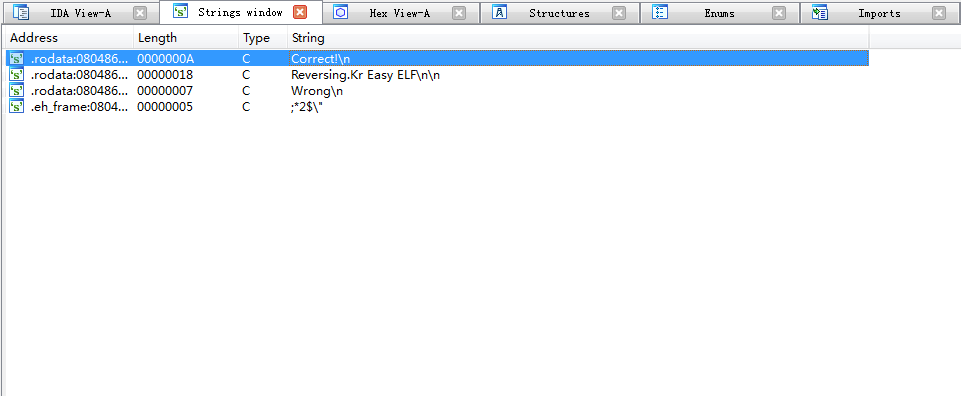
\includegraphics[width=10cm]{easyelf-str} \\
\item 双击 字符串“\lstinline$Correct!\n$”跳转到定义,发现在一个单独的函数内 \\
\item 右键 函数名,选择菜单项“Xrefs graph to...” \\
	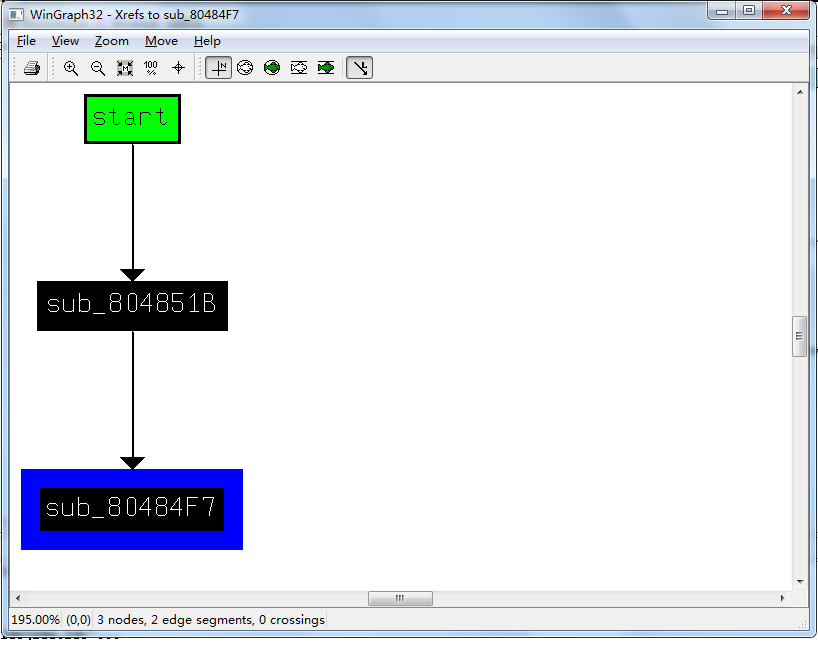
\includegraphics[width=10cm]{easyelf-call} \\
	在函数窗口双击 函数\lstinline$sub_80484F7$的父函数名称\lstinline$sub_804851B$,查看定义 \\
	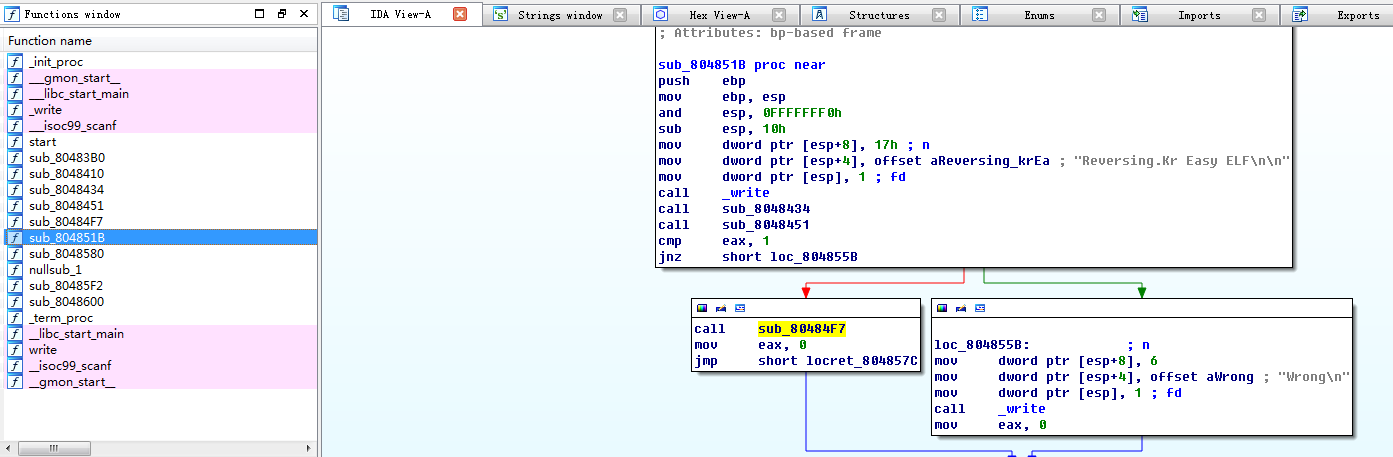
\includegraphics[width=15cm]{easyelf-judge} \\
	\begin{lstlisting}
	cmp     eax, 1
	jnz     short loc_804855B
	\end{lstlisting}
	预期eax值为1,才能走到正确的分支 \\
	\begin{lstlisting}
	call    sub_8048434
	call    sub_8048451
	\end{lstlisting}
	分析之前两个函数调用,第一个函数简单,是获取输入字符串存储至\lstinline$byte_804A020$,\\
	第二个函数是判断逻辑,返回值预期为1(eax值)\\
	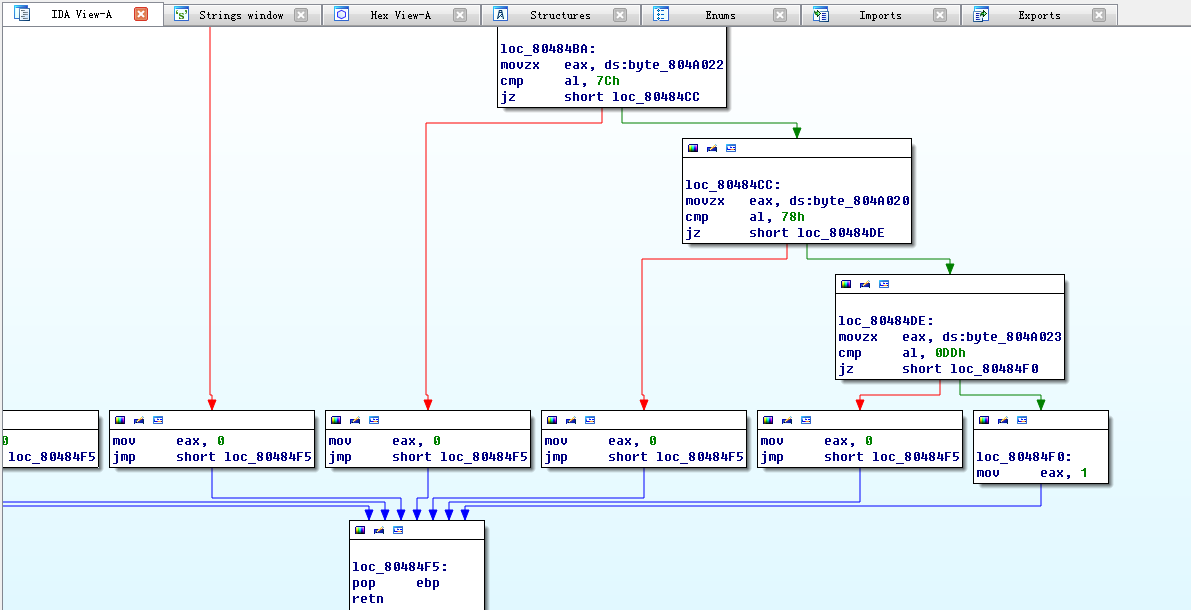
\includegraphics[width=15cm]{easyelf-cmp2} \\
	沿右侧绿色箭头指向,从后往前分析:\\
	\lstinline$byte_804A023$预期值是\lstinline$0DDh$ \\
	\lstinline$byte_804A020$预期值是\lstinline$78h$ \\
	\lstinline$byte_804A022$预期值是\lstinline$7Ch$ \\
	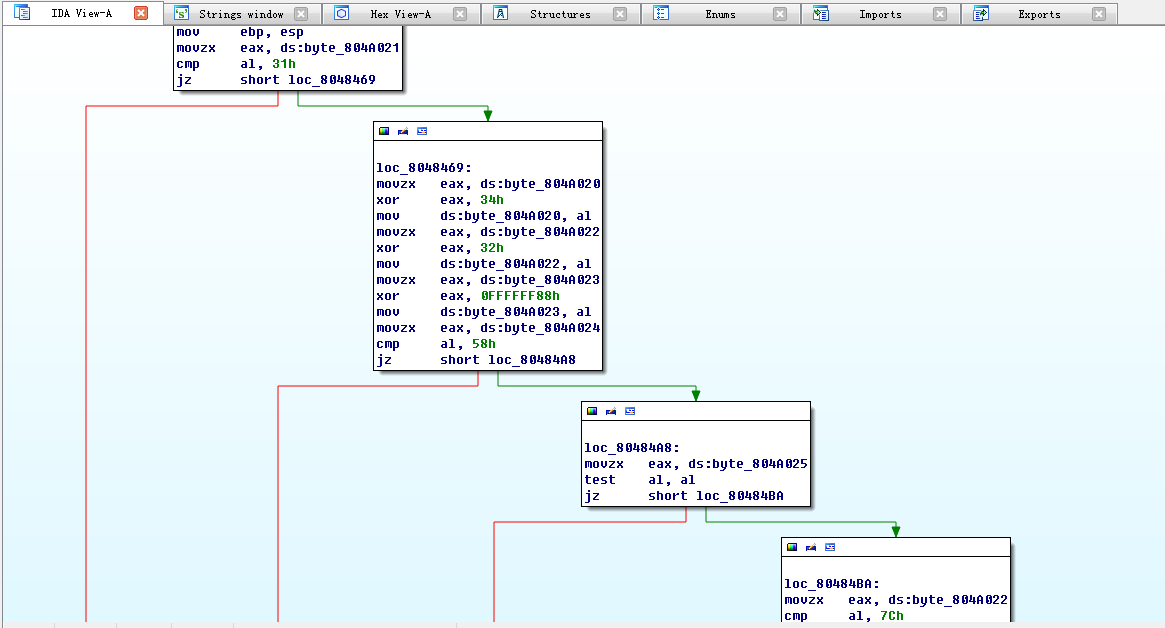
\includegraphics[width=15cm]{easyelf-cmp1} \\
	\lstinline$byte_804A025$预期值是\lstinline$00h$ \\
	\lstinline$byte_804A024$预期值是\lstinline$58h$ \\
	\lstinline$byte_804A023$转换为其值与\lstinline$0FFFFFF88h$进行异或的结果\\
	\lstinline$byte_804A022$转换为其值与\lstinline$32h$进行异或的结果\\
	\lstinline$byte_804A020$转换为其值与\lstinline$34h$进行异或的结果\\
	\lstinline$byte_804A021$预期值是\lstinline$31h$ \\
	整理一下分析结果:\\
	\lstinline$byte_804A020$ 异或 \lstinline$34h$ 结果预期值是\lstinline$78h$\\
	\lstinline$byte_804A021$预期值是\lstinline$31h$ \\
	\lstinline$byte_804A022$ 异或 \lstinline$32h$ 结果预期值是\lstinline$7Ch$\\
	\lstinline$byte_804A023$ 异或 \lstinline$88h$ 结果预期值是\lstinline$0DDh$\\
	\lstinline$byte_804A024$预期值是\lstinline$58h$ \\
	\lstinline$byte_804A025$预期值是\lstinline$00h$ \\
	将预期值反过来操作,得出原始输入字符串:\\
	\begin{lstlisting}[language=C]
	#include "stdio.h"
	int main()
	{
		char salt[5] = {0x34, 0x00, 0x32, 0x88, 0x00};
		char inputs[5] = {0x78, 0x31, 0x7C, 0xDD, 0x58};
		int i = 0;
		for (; i < 5; i++)
			printf("%c", inputs[i] ^ salt[i]);
		printf("\n");
	}
	\end{lstlisting}
	flag : ``L1NUX''
\end{enumerate}